% This file was created by tikzplotlib v0.9.8.
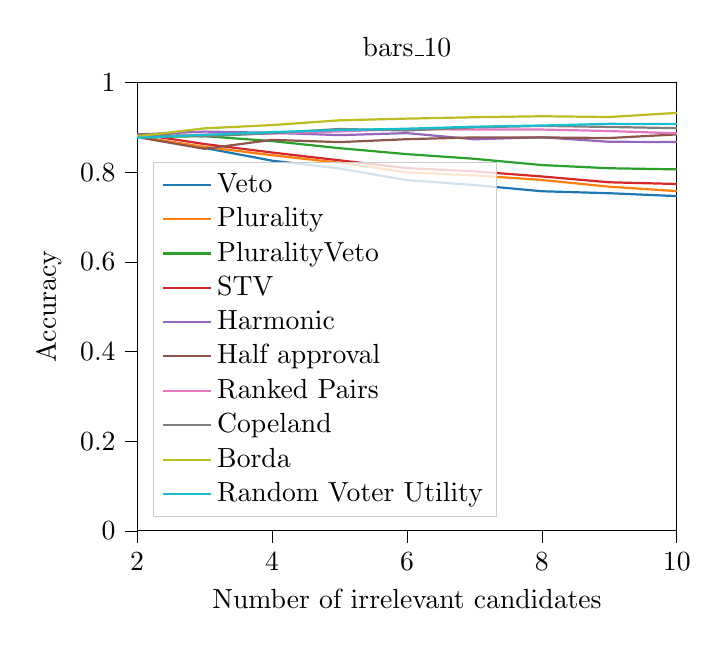
\begin{tikzpicture}

\definecolor{color0}{rgb}{0.12156862745098,0.466666666666667,0.705882352941177}
\definecolor{color1}{rgb}{1,0.498039215686275,0.0549019607843137}
\definecolor{color2}{rgb}{0.172549019607843,0.627450980392157,0.172549019607843}
\definecolor{color3}{rgb}{0.83921568627451,0.152941176470588,0.156862745098039}
\definecolor{color4}{rgb}{0.580392156862745,0.403921568627451,0.741176470588235}
\definecolor{color5}{rgb}{0.549019607843137,0.337254901960784,0.294117647058824}
\definecolor{color6}{rgb}{0.890196078431372,0.466666666666667,0.76078431372549}
\definecolor{color7}{rgb}{0.737254901960784,0.741176470588235,0.133333333333333}
\definecolor{color8}{rgb}{0.0901960784313725,0.745098039215686,0.811764705882353}

\begin{axis}[
legend cell align={left},
legend style={
  fill opacity=0.8,
  draw opacity=1,
  text opacity=1,
  at={(0.03,0.03)},
  anchor=south west,
  draw=white!80!black
},
tick align=outside,
tick pos=left,
title={bars\_10},
x grid style={white!69.0196078431373!black},
xlabel={Number of irrelevant candidates},
xmin=2, xmax=10,
xtick style={color=black},
y grid style={white!69.0196078431373!black},
ylabel={Accuracy},
ymin=0, ymax=1,
ytick style={color=black}
]
\addplot [thick, color0]
table {%
2 0.8801
3 0.854
4 0.8256
5 0.8082
6 0.7822
7 0.7713
8 0.7574
9 0.753
10 0.7466
};
\addlegendentry{Veto}
\addplot [thick, color1]
table {%
2 0.8789
3 0.8564
4 0.8378
5 0.821
6 0.7996
7 0.7928
8 0.7826
9 0.7676
10 0.7577
};
\addlegendentry{Plurality}
\addplot [thick, color2]
table {%
2 0.878
3 0.8803
4 0.8693
5 0.8535
6 0.8402
7 0.8298
8 0.8158
9 0.8087
10 0.8062
};
\addlegendentry{PluralityVeto}
\addplot [thick, color3]
table {%
2 0.8854
3 0.8627
4 0.8438
5 0.8264
6 0.809
7 0.8018
8 0.7904
9 0.7774
10 0.7736
};
\addlegendentry{STV}
\addplot [thick, color4]
table {%
2 0.884
3 0.8905
4 0.8878
5 0.8826
6 0.8871
7 0.8733
8 0.8779
9 0.8677
10 0.8673
};
\addlegendentry{Harmonic}
\addplot [thick, color5]
table {%
2 0.8782
3 0.8521
4 0.872
5 0.867
6 0.8735
7 0.8776
8 0.8774
9 0.8761
10 0.8842
};
\addlegendentry{Half approval}
\addplot [thick, color6]
table {%
2 0.8784
3 0.8838
4 0.8861
5 0.8909
6 0.8963
7 0.8949
8 0.895
9 0.8917
10 0.8866
};
\addlegendentry{Ranked Pairs}
\addplot [thick, white!49.8039215686275!black]
table {%
2 0.8843
3 0.8799
4 0.8869
5 0.8964
6 0.8929
7 0.8998
8 0.9032
9 0.9008
10 0.8981
};
\addlegendentry{Copeland}
\addplot [thick, color7]
table {%
2 0.88
3 0.8977
4 0.905
5 0.9156
6 0.9194
7 0.9225
8 0.9247
9 0.923
10 0.9322
};
\addlegendentry{Borda}
\addplot [thick, color8]
table {%
2 0.8766
3 0.8831
4 0.8893
5 0.894
6 0.8969
7 0.9014
8 0.904
9 0.9078
10 0.9071
};
\addlegendentry{Random Voter Utility}
\end{axis}

\end{tikzpicture}
